 \documentclass[11pt,a4paper]{article}
\usepackage[a4paper,margin=2cm]{geometry}
\usepackage[]{graphicx}
\usepackage{bm}
\usepackage[strings]{underscore}
\usepackage{apacite}
\bibliographystyle{apacite}
\usepackage{svg}
\usepackage{amsmath}
\setlength{\parindent}{0pt}
\graphicspath{ {./images} }
\usepackage{wrapfig}
\usepackage{float}
\usepackage[autostyle, english = american]{csquotes}
\usepackage[toc,page]{appendix}
\usepackage{amssymb}
\MakeOuterQuote{"}
\usepackage[T1]{fontenc}
\svgpath{./Diagrams}
\renewcommand{\baselinestretch}{1.2}
\begin{document}
\nocite{*}
\begin{titlepage}


\title{Determining the relationship between masses in equilibrium and the angle of a frictionless plane}

\author{Noah Alexiou}


\date{May 2025}

\maketitle
\centering

\end{titlepage}
\tableofcontents
\newpage

\section{Introduction}

\subsection{Research Question}
When the mass of an on a frictionless plane is altered, and the mass of a hanging object adjusted so equilibrium is achieved, what is the precision and uncertainty of this method in comparison to conventional measuring techniques? 

\subsection{Rationale}

The original experiment was conducted to determine the relationship between the mass of a carriage ($C_m$) and a hanging mass ($H_m$) when a frictionless plane was inclined at different angles. The results confirmed the theoretical relationship $H_m = C_m \sin(\theta)$.

It was noticed during the experiment that the angle measurement device, an `angle gun', had a large uncertainty ($\pm0.5\deg$) compared to the scale used to measure masses ($\pm0.005$ grams). It was questioned whether the relationship between the masses in equilibrium could be used to determine the angle of the plane with improved precision and uncertainty. 
\newline
\begin{figure}[h]
	\centering
	\includegraphics[width=0.5\paperwidth]{./Diagrams/set_upV2.png}
	\caption{Diagram of experimental setup}
\end{figure}
\newline
Considering Newtons first law, under equilibrium the net force is 0 \cite{encyclopediabritannica_2023_newtons}. This implies that under equilibrium,  $C_{f\parallel}=H_f$.

By plotting the experimental results of the experiment in Excel, a line of best fit can be determined. Since the relationship between the masses is established to be linear, we can use the gradient as a parameter to calculate the angle. 

\begin{center}
	\begin{align*}
	H_m= &\;C_m\cdot{\sin(\theta)} \\
	C_m= &\;H_m\cdot\frac{1}{{\sin(\theta)}}\;\;\;\; \;\;\;\;\;\because \textrm{Make dependent variable subject} \\
	\frac{C_m}{H_m}=&\;\textrm{gradient}	\;\;\;\;\;\;\;\;\;\;\;\;\;\;\because \textrm{gradient}=\frac{\textrm{rise}}{\textrm{run}}\\
\linebreak
	\frac{H_m}{C_m}=&\;\frac{1}{\mathrm{gradient}}=\sin(\theta) \because \sin(\theta)=\frac{O}{H}\\
	\therefore  \;\theta=&\;\sin^{-1}\left(\frac{1}{\textrm{gradient}}\right)
	\end{align*}
\end{center}


Since the angle is now expressed in terms of the gradient, the maximum and minimum slopes derived from experimental data can be used to determine the uncertainty in the angle by calculating the angle using each one of these extremes, then dividing the difference between them by $2$.




\subsection{Methodology}

\subsubsection{Modifications}


The following modifications to the method were implemented
\begin{itemize}
	\item The plane was kept at a constant angle throughout the entire duration of the experiment. This was done to isolate it from the independent and dependent variables and ensure that the results of all trials would point to the same relationship between them and the angle.
	\item The independent variable became the hanging mass ($H_m$). Since this mass could be directly measured and processed without the use of trigonometric functions, the only uncertainty in it's value should be random error from the scale. By conducting multiple trials with the same parameters, random error can be negated significantly. 
	\item The dependent variable became the carriage mass ($C_m$) as the large area inside each carriage allowed for fine adjustment of its mass via the addition of brass weights. 
\end{itemize}

\subsubsection{Materials}
\begin{itemize}
	\item Angle gun 
	\item Frictionless plane
	\item Brass weights
	\item Blue tack 
	\item Scale
	\item Carriage
\end{itemize}

\subsubsection{Method}
\begin{enumerate}
\item Set up slope at a constant angle as shown in Figure 1. It will remain at this angle for the entire duration of the experiment. 
\item Set the hanging mass ($H_m$) to its minimum value initially.
\item Alter the mass of the carriage $(C_m)$ until equilibrium with the $H_m$ is achieved, i.e. The carriage remains stationary. 
\item If the carriage does not have sufficient space for more weight, replace with a larger carriage or link an additional carriage to the chain.  
\item Measure and record masses. 
\item Repeat for 3 trials with current $H_m$ value.
\item Increase $H_m$ by 50 grams. 
\item Repeat until $H_m\geq\approx 300$g or until equilibrium cannot be achieved with equipment.
\end{enumerate}


\subsubsection{Risk Assessment}
\textbf{Frictionless plane}
\begin{itemize}
	\item Mishandling of heavy masses on the frictionless plane could result in them sliding down the slope at high speed. This could damage equipment of cause injury. The blower fan will be turned off not required, and one person will always be supporting the carriage whenever possible to prevent this.
	\item Using too low fan speed on the frictionless plane may not create enough of an air pocket to support heavy weights. This could create friction between the surfaces, which could damage equipment and introduce inaccuracies. The fan will be set to the highest possible speed throughout the experiment to negate the possibility of this occurring.
\end{itemize}
\textbf{Blower}
\begin{itemize}
	\item Leaving the blower fan on for extended periods may cause overheating, as clearly stated in its instructions. This further implies the need for the blower to be turned off when not required.
\end{itemize}
\textbf{Masses}
\begin{itemize}
	\item Heavy masses or items containing many brass weights may cause injury if dropped or mishandled. participants will wear enclosed footwear to negate injury if this occurs.  
\end{itemize}
\section{Results and Evaluation}
\subsection{Results}

\subsubsection{Raw Data}
\begin{center}
	\centering
	\begin{figure}[h]
		\centering
		\includegraphics[width=0.84\paperwidth]{resultstable.png}
		\caption{Raw results with additional calculations}
	\end{figure}
	
\end{center}


\subsubsection{Sample Calculations}
\begin{center}
\textbf{Absolute uncertainty for $C_m$ when $H_m=50.160$}
\begin{align*}
	\sigma(C_m)=&\pm\frac{\textrm{max}-\textrm{min}}{2}\\
	=&\pm\frac{139.20-138.55}{2}
	\\=&\pm0.325
\end{align*}
\newline

\textbf{Average mass of $C_m$ when $H_m=50.16$}
\begin{align*}
	\bar{C_m}=&\frac{\Sigma^n_{i=1}C_m}{n}\\
	=&\frac{138.55+139.20+138.54}{3}\\
	=&137.76
\end{align*}
\end{center}


\subsubsection{Prerequisite trigonometric measurements}

\begin{figure}[H]
	\centering

	\begin{tabular}{|l|l|l|}
		\hline
		\textbf{Hypotenuse} & \textbf{Length} & \textbf{Height} \\ \hline
		2.65       & 2.50   & 0.98   \\ \hline
	\end{tabular}

	\caption{Table showing the side lengths of triangle formed by incline plane}
\end{figure}


\begin{figure}[H]
	\centering
	\includegraphics[width=0.35\paperwidth]{./Diagrams/LengthDiagram.png}
	\caption{Diagram showing the side lengths of triangle formed by incline plane}
\end{figure}


\subsubsection{Plotting}

\begin{figure}[H]
\centering
\includegraphics[width=0.8\paperwidth]{newresults.png}
\caption{Average $H_m$ ($x$-axis) and $C_m$ ($y$-axis) extrapolated from experimental data}
\end{figure}




\section{Discussion}
\subsection{Analysis of evidence}
\subsubsection{Identification of trends}
Figure 5 depicts a clear linear relationship formed by the data plotted. This supports the previously investigated relationship  $H_m=C_m\cdot{\sin(\theta)}$. However, clearly this graph represents the rearranged equation $C_m=H_m\cdot \frac{1}{{\sin(\theta)}}$.


This can be confirmed by determining the ratio between each of its points:
\\

As $H_m$ doubles from $50.14$ to $100.06$, $C_m$ increases by a factor of $\frac{278.05}{138.76}=2.0038\approx2.00$

As $H_m$ doubles from $50.14$ to $100.06$, $C_m$ increases by a factor of $\frac{555.07}{278.05}=1.9963\approx2.00$

\hfill

The presence of vertical shift in the line of best fit implies there is some inaccuracy in the data. In theory the relationship should be directly proportional
To find the angle, the gradient of the slope of average values for each trial can be extrapolated from the line of best fit, and substituted into the equation found for angle in terms of gradient.

\begin{align*}
\centering
\;\theta=&\;\sin^{-1}\left(\frac{1}{\textrm{gradient}}\right)\\
 =& \;\sin^{-1}\left(\frac{1}{2.8266}\right)\\
	=&\;20.71881007^\circ
\end{align*}

\subsubsection{Uncertainty}

{\large \textbf{Finding uncertainty}\newline}
Since the value of $H_m$ was deliberately set, any uncertainty was due to the inherent random error in the scale used to measure it. By averaging $H_m$ across trials, a more reliable value can be found, however it should be noted that although this negates the effect of random error, the systematic uncertainty ($\pm0.005g$) is not affected as it is determined by the scale's precision.

To find the absolute uncertainty in the gradient, the maximum and minimum slopes were required. By considering the two average carriage masses with the largest uncertainties, say $m_1, m_2$, then plotting the line between $m_1+\sigma_1$ and $m_2-\sigma_2$, then  $m_1-\sigma_1$ and $m_2+\sigma_2$, the equations of the maximum and minimum slopes could be solved as the line of best fit.
\begin{center}
	\textbf{Absolute uncertainty in the gradient}
	\begin{align*}
		\centering
		\sigma(\textrm{gradient})=&\pm\frac{\textrm{max}-\textrm{min}}{2}\\
		\therefore\;\sigma(\textrm{gradient})=&\pm\frac{2.8643-2.7927}{2}\\
		=&\pm\frac{0.0716}{2}\\
		=&\pm0.0358
	\end{align*}
	
	\textbf{Absolute uncertainty in the angle}
	
	\begin{align*}
		\centering
		\sigma(\textrm{angle})=&\pm\frac{\textrm{max}-\textrm{min}}{2}\\
		\sigma(\textrm{angle})=&\pm\frac{\sin^{-1}(\frac{1}{2.8643})-\sin^{-1}(\frac{1}{2.7927})}{2}\\
		=&\pm0.274138198466^\circ 
	\end{align*}
	
\end{center}
\hfill

{\large \textbf{Possible sources of uncertainty}}



\textbf{Angle consistency}\newline
Since the experiment was conducted over multiple class periods, the experimental setup was dismantled and reassembled mid way through. Additionally the plane was bumped on multiple occasions, requiring it to be returned back to its original location and angle. Despite the angle of the plane measuring the same throughout the experiment, the uncertainty in the tool used to set the angle of the plane ($\pm0.5^\circ$) meant that the angle was likely inconsistent. This was not accounted for in any way.

\textbf{Friction}\newline
It was assumed that the frictionless plane was completely frictionless. This was not the case, and multiple factors likely altered the degree of friction across it throughout the experiment. 
It was noticed that when masses were in equilibrium, pushing the cart would cause it to move for a while, then slow down and stop. If the plane was truly frictionless then the plane would not have slowed down, but continued until it reached the end stop. It was theorised that the surface area of the carriage on the plane determined how much of an air pocket could form underneath it. This was briefly investigated as the type of carriage used was recorded for each trial. Considering one big carriage having the approximate equivalent surface area of two small carriages, the average uncertainty for each carriage surface area was graphed. However, rather than a reduction in uncertainty as surface area increased, an increase was observed. 
\begin{figure}[h]
	\centering
	\includegraphics[width=0.7\paperwidth]{./images/ApproxCarriage.png}
	
\end{figure}


\section{Evaluation}

\subsection{Reliability and validity}

As previously mentioned, the line of best fit constructed by the data did not cross through the origin, which implies error in the experimental process.

Talk about how calculating max and min normally resulted in max that was smaller than average...?

Using the lengths of each side of the right angle triangle formed by the incline plane and the ground, the angle between then can be found. It was found that the angle differed based on which trigonometric function was used. 
 
 \begin{align*}
 	\sin^{-1}\left({\frac{0.98}{2.64}}\right)=&\;21.79^\circ\\
 	\cos^{-1}\left({\frac{2.50}{2.64}}\right)=&\;18.74^\circ\\
 	\tan^{-1}\left({\frac{0.98}{2.50}}\right)=&\;21.41^\circ\\
 \end{align*}
 
 This indicates error in the measurement process. While assuming these values are equally reliable, then averaging them, would give a valid angle, this process introduces uncertainty. It was decided that the most reliable values were the hypotenuse since it was the length of the incline plane and physically could not have changed, and the vertical measurement taken from the top of the plane to the ground, as it was the easiest to confirm as parallel during the measurement process.
 
 Considering the ruler only measured in half centimetre increments, its uncertainty was $\pm 0.25$cm, or $\pm0.0025$m. By considering the sine value of $\frac{2.64-\sigma}{0.98+\sigma}$, and $\frac{2.64+\sigma}{0.98-\sigma}$, the absolute uncertainty in this measurement can be found.
 \begin{align*}
 	 \sin^{-1}\left(\frac{0.98+0.0025}{2.64-0.0025}\right)=&\;21.87\\
 	 \sin^{-1}\left(\frac{0.98-0.0025}{2.64+0.0025}\right)=&\;21.71\\
 \end{align*}

 \begin{align*}
 	\sigma=&\;\frac{\textrm{max}-\textrm{min}}{2}
 	\\
 	=&\;\frac{21.87-21.71}{2}
 	\\
 	=&\;\pm0.08
 \end{align*}

 
 
 Therefore the angle of the slope as determined via trigonometry was $\sin\left({\frac{0.98}{2.64}}\right)=\;21.79^\circ \pm0.08$




\subsection{Extension}



\section{Conclusion}
\newpage

\bibliography{./Bibliography/Physics_IA2.bib}

	
\end{document}